\chapter{Extending QuTiP with Quantum Information Functionality}
\chaptermark{Extending QuTiP with QI Functionality}

Now we are ready to deal with the primary concern of this project: extending QuTiP with QI functionality, focusing in particular on quantum entanglement tests and measures. This chapter details the implementation of these functions. All the new functions written will be stored in a module \texttt{quantinf} to be easily accessible from other programs.
\par We start by importing the modules that we shall use as our base.
\begin{verbatim}
from qutip import *
import numpy as np
\end{verbatim}
For convenience we can import functions by name to avoid having to use the \texttt{module.function} convention when using them.
\begin{verbatim}
from numpy import log2
\end{verbatim}
\par We now start with the entanglement tests that we saw in chapter 3.
\section{Purity of Reduced DM}
The most primitive entanglement test we saw in chapter 1 is to check if the reduced density matrix of a bipartite state represents a mixed state. We saw that for entangled states, the reduced density matrix will always be mixed. Let us keep in mind though that this test only works if the joint density matrix is a pure state and fails for mixed states.
\par The logical structure of this function is such that it would make sense to divide it into many smaller functions so that the code is easily reusable. Hence we define separate functions for checking purity of complete and reduced density matrices and make them depend on each other as needed. The function that we are after is \texttt{ismixed\_reduced}. The others defined before it can be thought of as helper functions.
\begin{verbatim}
def purity(dm):
    """ Calculates trace of density matrix square
    
    Parameters
    ----------
    dm: qobj/array-like
        Input density matrix
    
    Returns
    -------
    purity:
        Purity of the state. 1 for pure, 0.5 for maximally mixed.
    
    """
    if dm.type == 'ket':
        dm = ket2dm(dm)
    if dm.type != 'oper':
        raise TypeError("Input must be a state ket or density matrix")
    purity = (dm**2).tr()
    return purity


def purity_of_reduced(rho):
    """ Calculates trace of reduced density matrix square
    
    Parameters
    ----------
    dm: qobj/array-like
        Input density matrix
    
    Returns
    -------
    purityreduced:
        Purity of the reduced DM. 1 for pure, 0.5 for maximally mixed.
    
    """
    
    rhopartial = ptrace(rho,0)
    purityreduced = purity(rhopartial)
    return purityreduced


def ispure(dm):
    """ Checks whether or not a density matrix represents a pure state
    
    Parameters
    ----------
    dm : qobj/array-like
        Density operator representing the state.
    
    -------
    pure : bool
        Whether or not the state is pure. True: Pure, False: Mixed.
    
    """
    
    if np.round(purity(dm),8) == 1:
        return True
    else:
        return False


def ismixed_reduced(dm):
    """ One way to check for entanglement is that the reduced density
    matrix is mixed. This function checks for that criterion.
    
    Parameters
    ----------
    dm : qobj/array-like
        Density operator representing the state.
    
    -------
    mixed : bool
        Whether or not the reduced DM is mixed. True: Mixed, False: Pure
    
    """
    
    if np.round(purity_of_reduced(dm),8) != 1:
        return True
    else:
        return False

\end{verbatim}
What we are basically doing in \texttt{ismixed\_reduced} is that we are taking the partial trace of the input density matrix with respect to B and then squaring it and taking its trace to see if the reduced DM is mixed. \texttt{ismixed\_reduced} will return \texttt{True} if the reduced DM is mixed and return \texttt{False} if it is pure.

\section{The Peres-Horodecki Criterion}
The Peres-Horodecki criterion is a more general and reliable test for checking entanglement. It works for both pure and mixed states. It involves taking the partial transpose of the joint density matrix with respect to one of the subsystems (say B) and checking for negative eigenvalues. If there is a negative eigenvalue then the state is entangled.
\begin{verbatim}
def peres_horodecki_bipartite(rho, mask=[0,1]):
    """ Tests the given bipartite state for Peres-Horodecki criterion
    
    Parameters
    ----------
    rho: qobj/array-like
        Density operator for the state
    mask: list of int, length 2
        mask used for partial transpose
    
    Returns
    -------
    isentangled: bool
        True for entangled, False for disentangled
    
    """
    if rho.type != 'oper':
        raise TypeError("Input must be a density matrix")
    rhopt = partial_transpose(rho,mask)
    rhopt_eigs = rhopt.eigenenergies()
    if min(rhopt_eigs) < 0:
        isentangled = True
    else:
        isentangled = False
    return isentangled
\end{verbatim}
This function will return \texttt{True} if a given density matrix represents an entangled state by the Peres-Horodecki criterion and return \texttt{False} otherwise.
\\
\par Now we implement some entanglement measures.
\section{Entropy of Entanglement}
Recall the definition of entropy of entanglement:
\begin{align*}
S(\rho_A) = - tr \{ \rho_A \log \rho_A \}
\end{align*}
where $\rho_A$ is the reduced density matrix for subsystem $A$, obtained by partial trace w.r.t. subsystem $B$.
\begin{verbatim}
def entropy_entg(rho, base=2):
    """ Calculates the entropy of entanglement of a density matrix
    
    Parameters:
    -----------
    rho : qobj/array-like
        Input density matrix
    base:
        Base of log
    
    Returns:
    --------
    ent_entg: Entropy of Entanglement
    
    """
    if rho.type == 'ket':
        rho = ket2dm(rho)
    if rho.type != 'oper':
        raise TypeError("Input must be density matrix")
    rhopartial = ptrace(rho,0)
    ent_entg = entropy_vn(rhopartial,base)
    return ent_entg
\end{verbatim}

\section{Linear Entropy of Entanglement}
Linear entropy of entanglement is the linear approximation to entropy of entanglement and is given by
\begin{align*}
S_L(\rho_A) = 1 - tr(\rho_A^2)
\end{align*}
where $\rho_A$ is obtained by a partial trace w.r.t. $B$.
\par To write the function for linear entropy of entanglement, we first need to write our own function for linear entropy which is more suited to the task than QuTiP's current implementation. Then we define a linear entropy of entanglement function based on that.
\begin{verbatim}
def linear_entropy(dm, normalize=False):
    """ Returns the linear entropy of a state.
    
    Parameters
    ----------
    dm : qobj/array-like
        Density operator representing the state.
    normalize : bool
        Optional argument to normalize linear entropy such that the
        completely mixed state has LE = 1 rather than 1-1/d. [1]
        Default: False
    
    ----------
    le : float
        Linear entropy
        
    ----------
    References:
        [1] "Linear entropy and Bell inequalities", Santos and Ferrero,
            Phys. Rev. A 62, 024101
    
    """
    if dm.type not in ('oper','ket'):
        raise TypeError("Input must be a Qobj representing a state.")
    if dm.type=='ket':
        dm = ket2dm(dm)
    
    le = 1 - (dm**2).tr()
    if normalize:
        d = dm.shape[0]
        le = le * d/(d-1)
    return le

def entropy_linear_entg(rho, normalize=True):
    """ Calculates the linear entropy of entanglement of a density matrix
    
    Parameters:
    -----------
    rho : qobj/array-like
        Input density matrix
    normalize : bool
        Optional argument to normalize linear entropy of entanglement
        such that the completely entangled state has value = 1.
        Default: True
    
    Returns:
    --------
    linent_entg: Linear Entropy of Entanglement
    
    """
    if rho.type == 'ket':
        rho = ket2dm(rho)
    if rho.type != 'oper':
        raise TypeError("Input must be density matrix")
    rhopartial = ptrace(rho,0)
    linent_entg = linear_entropy(rhopartial,normalize)
    return linent_entg
\end{verbatim}

\section{Renyi Entanglement Entropy}
Renyi entanglement entropy of a density matrix $\rho$ is
\begin{align*}
S_\alpha (\rho_A) &= \frac{1}{1-\alpha} \log \left( \sum_i q_i^\alpha \right) , \quad \alpha \neq 1 \: \text{and} \: \alpha > 0
\end{align*}
where $\alpha$ is the Reyi index and $q_i$ are the eigenvalues of the reduced density matrix.
\par Once again we define two separate functions to allow for maximum code reuse: one function to calculate the usual Renyi entropy of the whole density matrix and the other to pass the reduced density matrix to the former function.
\begin{verbatim}
def entropy_renyi(rho,alpha):
    """ Calculate Renyi entropy of the density matrix with given index
    (Currently limited to 2-level systems)
    
    Parameters
    ----------
    dm: qobj/array-like
        Input density matrix
        
    alpha: Renyi index alpha
    
    Returns
    -------
    ent_rn: Renyi Entropy
    
    """
    if rho.type != 'oper':
        raise TypeError("Input must be a density matrix")
    
    qi = rho.eigenenergies()
    
    if alpha == 1:
        ent_rn = entropy_vn(rho,2)
    elif alpha >= 0:
        ent_rn = ( 1/(1-alpha) ) * log2 ( sum( qi**alpha ) )
    else:
        raise ValueError("alpha must be a non-negative number")
    
    return ent_rn

def entropy_renyi_entg(rho,alpha):
    """ Calculate Renyi entropy of entanglement for the DM with given index
    (Currently limited to 2-level systems)
    
    Parameters
    ----------
    dm: qobj/array-like
        Input density matrix
        
    alpha: Renyi index alpha
    
    Returns
    -------
    ent_rn_entg: Renyi Entropy of Entanglement
    
    """
    rhopartial = ptrace(rho,0)
    ent_rn_entg = entropy_renyi(rhopartial,alpha)
    return ent_rn_entg

\end{verbatim}

\section{Negativity}
Negativity of a density matrix $\rho$ is given by
\begin{align*}
N(\rho) = \frac{\lVert \rho^{T_A} \rVert_1 - 1}{2}
\end{align*}
Implementing in QuTiP:
\begin{verbatim}
def negativity(rho,mask=[1,0]):
    """ Calculate the negativity for a density matrix
    
    Parameters:
    -----------
    rho : qobj/array-like
        Input density matrix
    
    Returns:
    --------
    neg : Negativity
    
    """
    
    if rho.type != 'oper':
        raise TypeError("Input must be a density matrix")
    rhopt = partial_transpose(rho,mask)
    neg = ( rhopt.norm() - 1 ) / 2
    return neg
\end{verbatim}

\section{Logarithmic Negativity}
Logarithmic negativity for a density matrix $\rho$ is given by
\begin{align*}
E_N(\rho) = log_2 \lVert \rho^{T_A} \rVert_1
\end{align*}
Implementing in QuTiP:
\begin{verbatim}
def log_neg(rho,mask=[1,0]):
    """ Calculate the logarithmic negativity for a density matrix
    
    Parameters:
    -----------
    rho : qobj/array-like
        Input density matrix
    
    Returns:
    --------
    logneg: Logarithmic Negativity
    
    """
    
    if rho.type != 'oper':
        raise TypeError("Input must be a density matrix")
    rhopt = partial_transpose(rho,mask)
    logneg = log2( rhopt.norm() )
    return logneg
\end{verbatim}


\section{Other Quantum Information Functions}
\par Some functions other than entanglement tests and measures were also implemented as part of exploration of the various QI toolboxes.
\subsection{Schmidt Decomposition}
If $\ket{\psi_{AB}}$ is a pure bipartite state and $\{\ket{i^A}\}$ and $\{\ket{j^B}\}$ are the bases for subsystems $A$ and $B$, then $\ket{\psi_{AB}}$ can be written as
\begin{align*}
\ket{\psi_{AB}} &= \sum_{i,j} \beta_{ij} \ket{i^A} \ket{j^B}
\end{align*}
where $\beta_ij$ is a complex number.
\par The Schmidt decomposition rewrites the state in two new bases $\{\ket{\psi_i^A}\}$ and $\{\ket{\phi_i^B}\}$ such that
\begin{align*}
\ket{\psi_{AB}} &= \sum_{i} \alpha_i \ket{\psi_i^A} \ket{\phi_i^B}
\end{align*}
Now the sum is only over one index $i$ which is easier to calculate.
\par To implement Schmidt decomposition, we take some hints from QETLAB and use the singular value decomposition function from NumPy's linear algebra module.
\begin{verbatim}
def schmidt_decomposition(vec):
    """ Schmidt decomposition of a bipartite vector
    Logic based on the implementation in QETLAB 0.9
    which was written by Nathaniel Johnston (nathaniel@njohnston.ca)
    and as of this port, last updated on December 1, 2012
    
    Parameters
    ----------
    vec : qobj, ket vector of product state
        ket vector representing the bipartite state
    
    -------
    Returns:
    [s, u, v]
    s : list of floats
        Schmidt coefficients
    u : list of Qobj
        list of left Schmidt vectors of ket
    v : list of Qobj
        list of right Schmidt vectors of ket
    
    """
    
    if vec.type != 'ket':
        raise TypeError("Input must be a ket vector.")
    if len(vec.dims[0])==1:
        raise TypeError("Input must be a joint state.")
    
    dim = vec.dims[0][0]
    vecnp = vec.full()
    vecnpr = np.reshape(vecnp,[dim,dim])
    um,s,vm = np.linalg.svd(vecnpr)
    
    s = list(s)
    
    def extract_vecs(mat):
        veclist = list()
        for j in range(mat.shape[1]):
            veclist.append(Qobj(mat[:,j]))
        return veclist
    u = extract_vecs(um)
    v = extract_vecs(vm)
    
    return [s,u,v]
\end{verbatim}

\subsection{Kullback-Leibler Distance}
The Kullback-Leibler distance - also known as relative entropy in quantum information - is a measure of distance between two density matrices. It is not a true distance measure because it is not symmetric. Nevertheless it is a useful function in quantum information theory as it generates a good entanglement measure when used in conjunction with relative entropy of entanglement (see section 3.7.7). \cite{vedralteleportation}
\begin{align*}
S(\rho||\sigma) &= tr ( \rho \log \rho - \rho \log \sigma )
\end{align*}
Implementing in code:
\begin{verbatim}
def dist_kl(rho, sgm):
    """ Calculates the Kullback-Leibler distance (a.k.a. relative entropy)
    between DMs rho and sgm representing two-level systems.
    
    Parameters
    ----------
    rho : qobj/array-like
        First density operator.

    sgm : qobj/array-like
        Second density operator.

    Returns
    -------
    kldist : float
        Relative Entropy between rho and sgm.

    Examples
    --------
    >>> 
    
    """
    
    if rho.type != 'oper' or sgm.type != 'oper':
        raise TypeError("Inputs must be density matrices..")
    
    ent_vn = entropy_vn(rho,2)
    
    r_eigs = rho.eigenenergies()
    s_eigs = sgm.eigenenergies()
    # too small negtive values may give trouble
    s_eigs = np.round(s_eigs,8)
    
    kldist = -ent_vn
    for pj, qj in zip(r_eigs,s_eigs):
        if qj==0:
            pass
        else:
            kldist -= pj * log2(qj)
            
    kldist = abs(kldist)
    return kldist
\end{verbatim}


\section{Example Usage of the New Functions}
We can now explore some example cases with the newly written QI functions.

\subsection{Time Evolution under a Joint Hamiltonian}
Let us go back to the example of two particles getting entangled as a result of time evolution under a joint Hamiltonian from section 5.2.3. This time we shall plot the different tests and measures of entanglement as the state evolves.
\begin{verbatim}
#!/usr/bin/env python
# -*- coding: utf-8 -*-
"""
Time Evolution under a Joint Hamiltonian

An initially separable state evolves under a joint Hamiltonian
and becomes entangled. This program plots various entanglement
tests and measures as the state evolves.

@author: Muhammad Saad <muhammad.saad@yandex.com>
"""

from qutip import *
import numpy as np
from matplotlib import pyplot as plt
import quantinf

h = basis(2,0)
v = basis(2,1)

psi_a = 1/np.sqrt(2) * ( h + v )
psi_b = 1/np.sqrt(2) * ( h + v )
psi_ab_t0 = tensor(psi_a,psi_b)
print("Original state of psi_ab at time t0 =\n",psi_ab_t0.full())
print()
rho_ab_t0 = ket2dm(psi_ab_t0)

hmlt = Qobj([[1,0,0,0],[0,1,0,0],[0,0,1,0],[0,0,0,-1]])
hmlt.dims = [[2, 2], [2, 2]]
print("Hamiltonian H =\n", hmlt.full())
print()

tf = np.pi/2
t = np.linspace(0,tf)

measures = {'ent_entg':None,'linent_entg':None,'neg':None,'logneg':None,
            'entrn_entg_2':None,'entrn_entg_3':None,'entrn_entg_4':None,
            'cncr':None,'entrel':None,'reducedmixed':None,'phcrit':None}

for i in measures:
    measures[i] = np.zeros(len(t))

for i in range(len(t)):
    hmltpr = (-1j*t[i]) * hmlt
    hmlt_tf = hmltpr.expm()
    psi_ab_tf = hmlt_tf * psi_ab_t0
    rho_ab_tf = ket2dm(psi_ab_tf)
    # Round off very small decimals
    measures['cncr'][i] = concurrence(rho_ab_tf)
    measures['ent_entg'][i] = quantinf.entropy_entg(rho_ab_tf)
    measures['linent_entg'][i] = quantinf.entropy_linear_entg(rho_ab_tf)
    measures['entrn_entg_2'][i] = quantinf.entropy_renyi_entg(rho_ab_tf,2)
    measures['entrn_entg_3'][i] = quantinf.entropy_renyi_entg(rho_ab_tf,3)
    measures['entrn_entg_4'][i] = quantinf.entropy_renyi_entg(rho_ab_tf,4)
    measures['neg'][i] = quantinf.negativity(rho_ab_tf)
    measures['logneg'][i] = quantinf.log_neg(rho_ab_tf)
    measures['entrel'][i] = \
                 quantinf.dist_kl(ptrace(rho_ab_tf,0),ptrace(rho_ab_t0,0))
    measures['reducedmixed'][i] = quantinf.ismixed_reduced(rho_ab_tf)
    measures['phcrit'][i] = quantinf.peres_horodecki_bipartite(rho_ab_tf)

print("Final operator at time tf (t0 + pi*hbar/2) =\n",hmlt_tf.full())
print()
print("Final state of psi_ab at time tf =\n", psi_ab_tf.full())
print()

# Font size for plot
fsz = 12
# Limit for x axis
xlm = [0,tf]
# Limit for y axis
ylm = [0,1]

plt.figure(1)
plt.suptitle("Comparison of measures and tests of entanglement",fontsize=14)
plt.subplots_adjust(hspace=.5)

plt.subplot(331)
plt.plot(t, measures['ent_entg'])
plt.xlabel("Time t",fontsize=fsz)
plt.ylabel("Entr. Entanglement",fontsize=fsz)
plt.title("Increase in Entropy of Entanglement",fontsize=fsz)
plt.xlim(xlm)
plt.ylim(ylm)
plt.grid(True)

plt.subplot(332)
plt.plot(t, measures['linent_entg'])
plt.xlabel("Time t",fontsize=fsz)
plt.ylabel("Lin. Entr. Entanglement",fontsize=fsz)
plt.title("Increase in Linear Entropy of Entanglement",fontsize=fsz)
plt.xlim(xlm)
plt.ylim(ylm)
plt.grid(True)

plt.subplot(333)
plt.plot(t, measures['entrn_entg_2'],'r-', label='alpha = 2')
plt.plot(t, measures['entrn_entg_3'],'b--', label='alpha = 3')
plt.plot(t, measures['entrn_entg_4'],'g:', label='alpha = 4')
plt.legend(loc='upper left', fontsize='small')
plt.xlabel("Time t",fontsize=fsz)
plt.ylabel("Renyi Entanglement Entropy",fontsize=fsz)
plt.title("Renyi Entanglement Entropy with diff. values of alpha",fontsize=fsz)
plt.xlim(xlm)
plt.ylim(ylm)
plt.grid(True)

plt.subplot(334)
plt.plot(t, measures['neg'])
plt.xlabel("Time t",fontsize=fsz)
plt.ylabel("Negativity",fontsize=fsz)
plt.title("Increase in Negativity",fontsize=fsz)
plt.xlim(xlm)
plt.ylim(ylm)
plt.grid(True)

plt.subplot(335)
plt.plot(t, measures['logneg'])
plt.xlabel("Time t",fontsize=fsz)
plt.ylabel("Log Negativity",fontsize=fsz)
plt.title("Increase in Logarithmic Negativity",fontsize=fsz)
plt.xlim(xlm)
plt.ylim(ylm)
plt.grid(True)

plt.subplot(336)
plt.plot(t, measures['entrel'])
plt.xlabel("Time t",fontsize=fsz)
plt.ylabel("K-L Distance",fontsize=fsz)
plt.title("Increase in K-L Dist. of rho_A from its original state",fontsize=fsz)
plt.xlim(xlm)
plt.ylim(ylm)
plt.grid(True)

plt.subplot(337)
plt.plot(t, measures['cncr'])
plt.xlabel("Time t",fontsize=fsz)
plt.ylabel("Concurrence",fontsize=fsz)
plt.title("Increase in Concurrence",fontsize=fsz)
plt.xlim(xlm)
plt.ylim(ylm)
plt.grid(True)

xlm = [-0.04,tf+0.02]
ylm = [-0.1,1.1]

plt.subplot(338)
plt.plot(t, measures['reducedmixed'], 'ro')
plt.xlabel("Time t",fontsize=fsz)
plt.ylabel("Entangled Status",fontsize=fsz)
plt.title("Entanglement Test: Reduced DM is Mixed",fontsize=fsz)
plt.xlim(xlm)
plt.ylim(ylm)
plt.grid(True)

plt.subplot(339)
plt.plot(t, measures['phcrit'], 'ro')
plt.xlabel("Time t",fontsize=fsz)
plt.ylabel("Entangled Status",fontsize=fsz)
plt.title("Entanglement Test: Peres-Horodecki Criterion",fontsize=fsz)
plt.xlim(xlm)
plt.ylim(ylm)
plt.grid(True)

plt.show()

\end{verbatim}
\par This program generates a number of plots for various tests and measures of entanglement as the state evolves in time. Time in these plots is measured in units of $\hbar$. Let us take a look at all of them individually.
\pagebreak
\subsubsection{Mixedness of the Reduced Density Matrix}
This plot shows whether or not the state of an individual subsystem (the reduced density matrix) is mixed at all stages in its evolution. We plot the result as \texttt{False = 0} or \texttt{True = 1}. \texttt{True} means that the reduced density matrix is mixed and \texttt{False} means the reverse.

\begin{center}
\begin{figure}[H]
  \begin{center}
    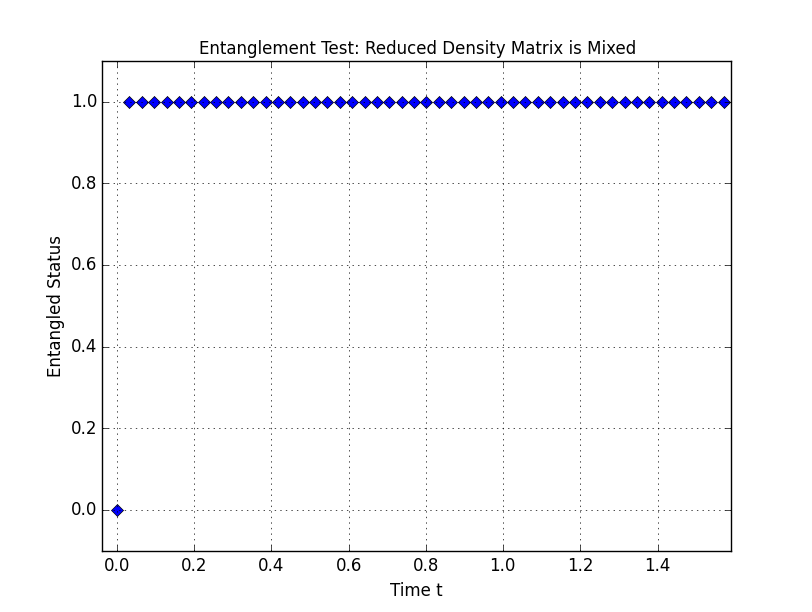
\includegraphics[scale=0.62]{figures/timeevolution-08.png}
    \caption{Checking for whether or not the reduced density matrix of the pair is mixed at various stages in the Hamiltonian evolution.\newline \texttt{0 = False = Separable,    1 = True = Entangled} }
    \label{fig: Time Evolution: Mixedness of Reduced DM}
  \end{center}
\end{figure}
\end{center}

This entanglement test has the limitation that it only works for pure states. However that is not a problem here because we are dealing with a pure state.
\par We see that the particles start getting entangled as soon as they start interacting with each other.


\pagebreak
\subsubsection{The Peres-Horodecki Criterion}
This is the plot of whether or not the state is entangled by the Peres-Horodecki criterion during all stages in its evolution. It follows the same convention: 0 represents \texttt{False} which means the state is separable; 1 represents \texttt{True} which means the state is entangled.

\begin{center}
\begin{figure}[H]
  \begin{center}
    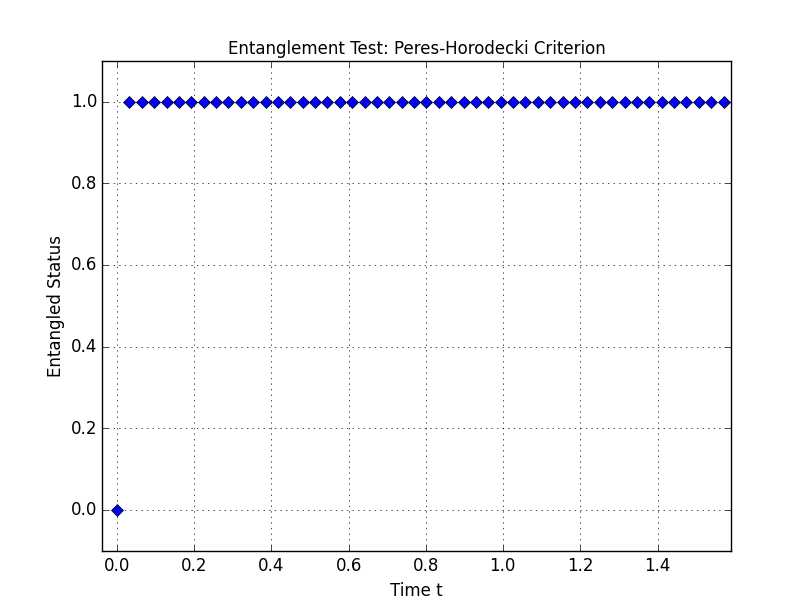
\includegraphics[scale=0.62]{figures/timeevolution-09.png}
    \caption{Checking the Peres-Horodecki criterion for entanglement at various stages in the Hamiltonian evolution.\newline \texttt{0 = False = Separable,    1 = True = Entangled}}
    \label{fig: Time Evolution: Peres-Horodecki Critetrion}
  \end{center}
\end{figure}
\end{center}

This entanglement test is more general and works well for both pure and mixed states.
\par We see that the particles start getting entangled as soon as they start interacting with each other.


\pagebreak
\subsubsection{Entropy of Entanglement and Linear Entropy of Entanglement}
The particle pair starts off with a disentangled state. Both the entropy of entanglement and the relative entropy of entanglement at time $t=0$ are zero as expected. As the state evolves and gets entangled, both of the entropies start increasing and reach their maximum values at time $t=\pi\hbar/2$. These two graphs display the trend of increase for both.

\begin{center}
\begin{figure}[H]
  \begin{center}
    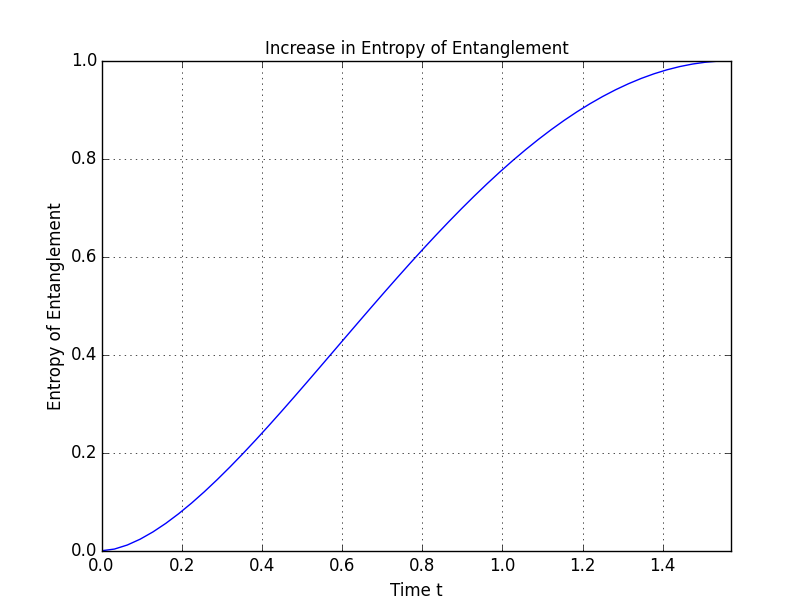
\includegraphics[scale=0.62]{figures/timeevolution-01.png}
    \caption{Increase in the entropy of entanglement of the bipartite state as it evolves under a joint Hamiltonian}
    \label{fig: Time Evolution: Entropy of Entanglement}
  \end{center}
\end{figure}
\end{center}

\begin{center}
\begin{figure}[H]
  \begin{center}
    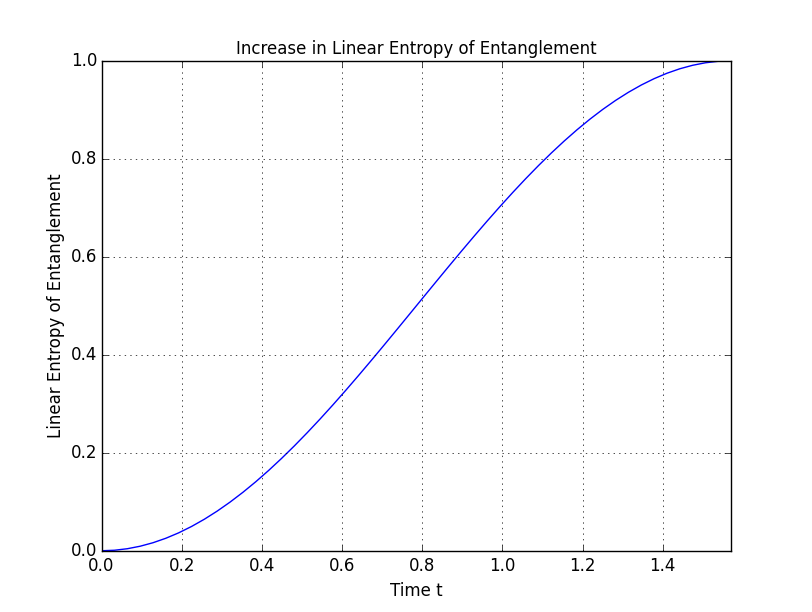
\includegraphics[scale=0.62]{figures/timeevolution-02.png}
    \caption{Increase in the linear entropy of entanglement of the bipartite state as it evolves under a joint Hamiltonian}
    \label{fig: Time Evolution: Linear Entropy of Entanglement}
  \end{center}
\end{figure}
\end{center}

The linear entropy of entanglement in this example is calculated with \texttt{normalize=True}, which normalizes it so that the completely entangled state has value 1 rather than $(1-\frac{1}{d})$ \cite{linentropybellineq}. We see that the linear entropy of entanglement closely traces the same path as the entropy of entanglement, since it is a linear approximation, and becomes 1 for the maximally entangled state.

\pagebreak
\subsubsection{Renyi Entanglement Entropies}
The Renyi entanglement entropies start with zero at the disentangled state. As the state evolves, they increase and finally reach the maximum value for the maximally entangled state.
\begin{figure}[H]
  \begin{center}
    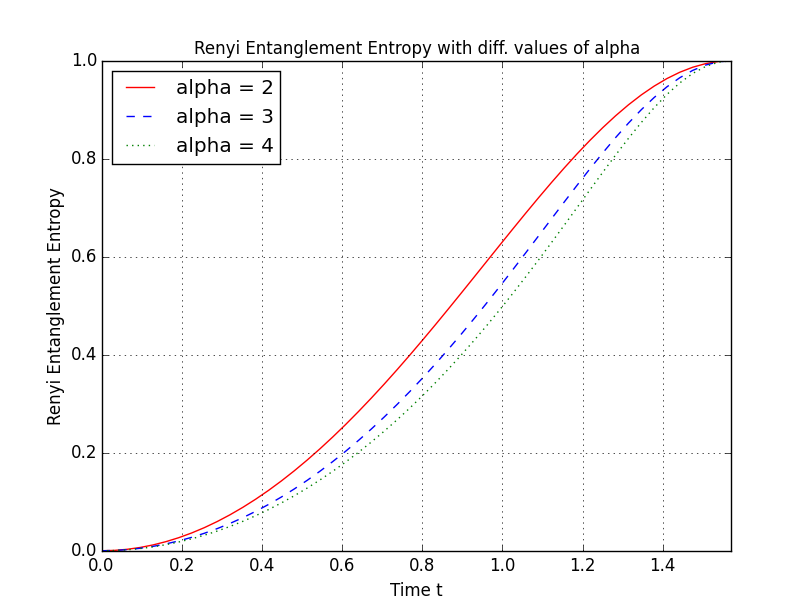
\includegraphics[scale=0.62]{figures/timeevolution-03.png}
    \caption{Increase in the Renyi entanglement entropies of the bipartite state for various values of $\alpha$}
    \label{fig: Time Evolution: Renyi Entanglement Entropies}
  \end{center}
\end{figure}

We observe that the minimum and maximum values for all values of $\alpha$ are the same: 0 and 1 respectively. With increasing value of $\alpha$, the curve shifts to the right.
\par Let us look at the Renyi entanglement entropies for a continuous range of $\alpha$ in the following 3-dimensional plot.

\begin{figure}[H]
  \begin{center}
    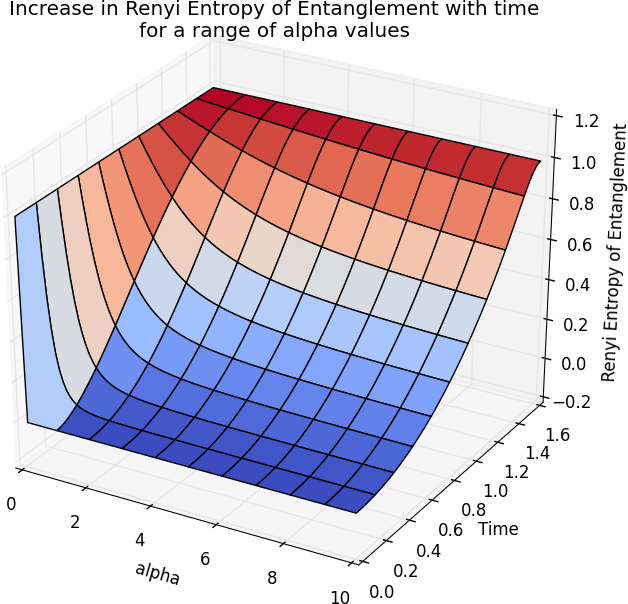
\includegraphics[scale=0.68]{figures/renyi-entg-3d.png}
    \caption{Increase in Renyi entanglement entropies with time for a range of values of $\alpha$. Time ranges from 0 to $\pi\hbar/2$ and $\alpha$ ranges from 0 to 10. Z-axis represents the Renyi entanglement entropies for all the combinations.}
    \label{fig: Time Evolution: Renyi Entanglement Entropies (3D)}
  \end{center}
\end{figure}

We observe the same trend for increasing value of $\alpha$. If we single out the curve for $\alpha=1$, we will find that it is the same as the entropy of entanglement.


\pagebreak
\subsubsection{Negativity and Logarithmic Negativity}
Negativity and logarithmic negativity both start at zero for the disentangled state. As the state evolves, they increase and reach their maximum values for the maximally entangled state.

\begin{center}
\begin{figure}[H]
  \begin{center}
    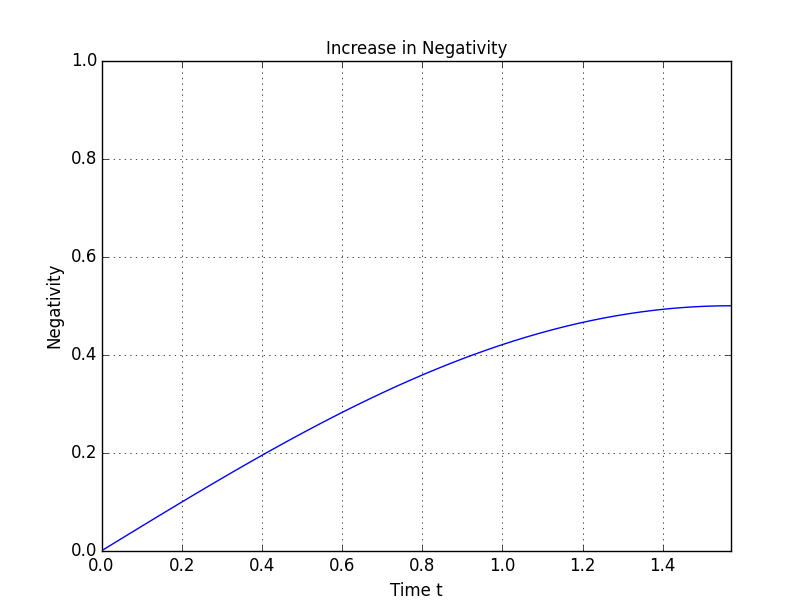
\includegraphics[scale=0.62]{figures/timeevolution-04.png}
    \caption{Increase in negativity of the bipartite state}
    \label{fig: Time Evolution: Negativity}
  \end{center}
\end{figure}
\end{center}

Negativity of the state starts at 0 when the pair is disentangled. As the state evolves, negativity gradually increases until it reaches 0.5 for the maximally entangled bipartite state.

\begin{center}
\begin{figure}[H]
  \begin{center}
    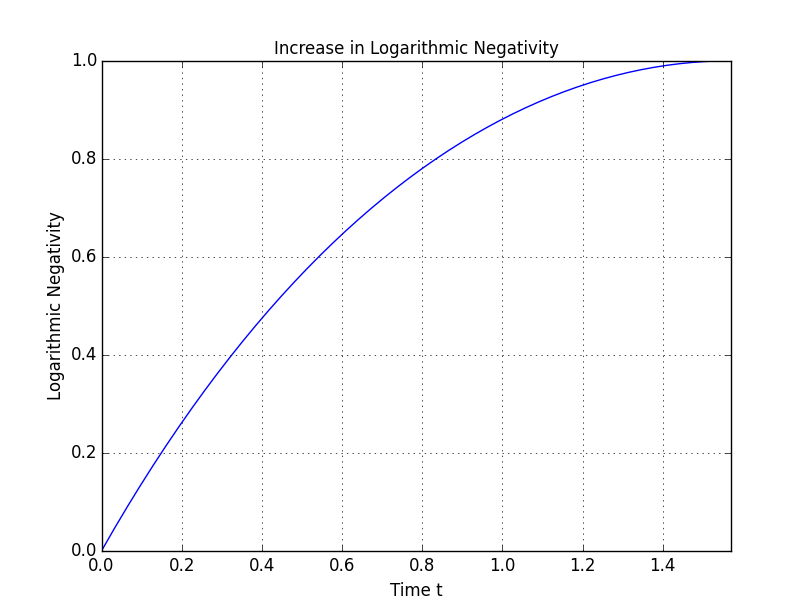
\includegraphics[scale=0.62]{figures/timeevolution-05.png}
    \caption{Increase in logarithmic negativity of the bipartite state}
    \label{fig: Time Evolution: Logaritmic Negativity}
  \end{center}
\end{figure}
\end{center}

Logarithmic negativity is an entanglement measure based on negativity that in addition has the additivity property. This plot illustrates the trend for increase in logarithmic negativity as it starts with 0 for the disentangled state and reaches a maximum value of 1 for the maximally entangled state.


\pagebreak
\subsubsection{Kullback-Leibler Distance}
The Kullback-Leibler distance can be used for defining an entanglement measure by searching over the space of all possible separable states. However here for simplicity we take a different route. We measure the KL-distance of one of the subsystems with respect to its original disentangled state to see how it changes in time. Please note that this particular graph \textit{does not} show an entanglement measure. It is just a speculative experiment.

\begin{center}
\begin{figure}[H]
  \begin{center}
    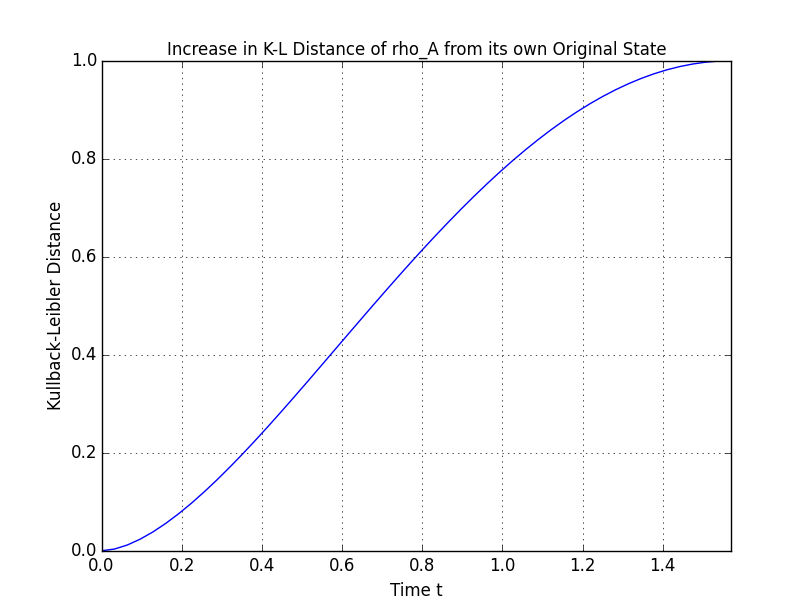
\includegraphics[scale=0.62]{figures/timeevolution-06.png}
    \caption{As the bipartite system evolves under the joint Hamiltonian, the Kullback-Leibler distance of both subsystems $\rho_A$ and $\rho_B$ with respect to their respective original states increases. This indicates that the density matrix of each subsystem is evolving and becoming different from what it was.}
    \label{fig: Time Evolution: Kullback-Leibler Distance}
  \end{center}
\end{figure}
\end{center}

To use (computationally) the Kullback-Leibler distance for defining an entanglement measure, we will have to generate the set of all possible separable states and compute the distances from our state $\rho_{AB}$ to each of them. The minimum of these distances will give the \textit{relative entropy of entanglement} for our joint density matrix $\rho_{AB}$.


\pagebreak
\subsubsection{Concurrence}
To compute concurrence, the function \texttt{concurrence} already available in QuTiP has been used. This plot illustrates the increasing trend in concurrence under the Hamiltonian evolution in question.

\begin{center}
\begin{figure}[H]
  \begin{center}
    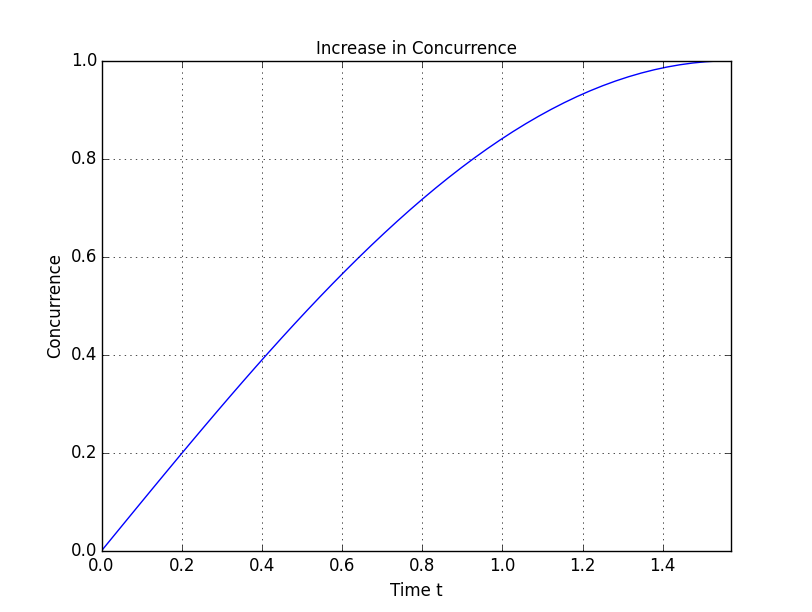
\includegraphics[scale=0.62]{figures/timeevolution-07.png}
    \caption{Increase in concurrence of the bipartite state under joint Hamiltonian evolution}
    \label{fig: Time Evolution: Concurrence}
  \end{center}
\end{figure}
\end{center}

We observe that concurrence starts with zero for the disentangled state and becomes 1 for the maximally entangled state.

\pagebreak
\subsubsection{What Happens After Time $\pi\hbar/2$?}
It should be noted that the plot upto time $\pi\hbar/2$ is not the complete picture. The system does not stay constantly at the point of maximum entanglement under this Hamiltonian evolution. We can observe changes in the amount of entanglement if we increase the time interval from $\pi\hbar/2$.
\par For example, here is the plot of concurrence from 0 to $3\pi\hbar$.

\begin{center}
\begin{figure}[H]
  \begin{center}
    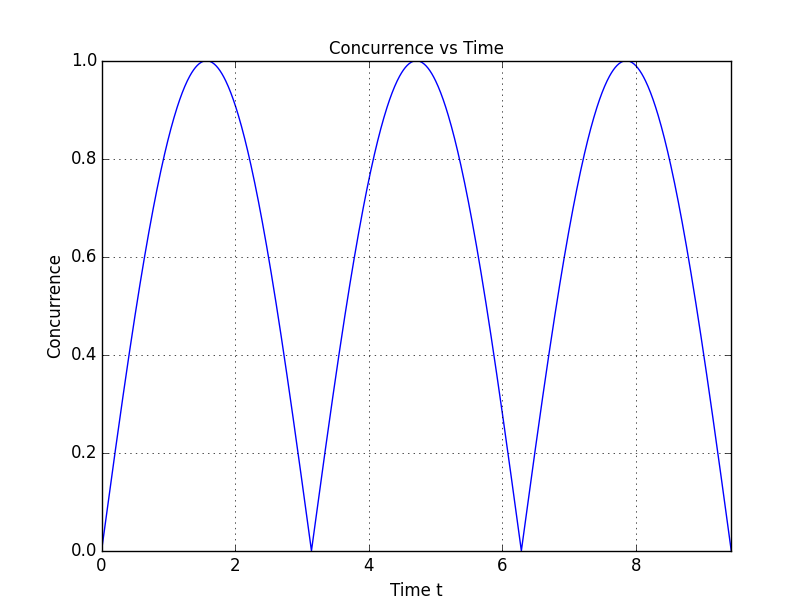
\includegraphics[scale=0.62]{figures/timeevolution-10.png}
    \caption{Concurrence as a function of time under joint Hamiltonian evolution, time ranging from 0 to $3\pi\hbar$. \newline We see that the state keeps oscillating between entangled and disentangled. At times which are multiples of $\pi\hbar$, the state becomes disentangled again.}
    \label{fig: Time Evolution: Concurrence (extended)}
  \end{center}
\end{figure}
\end{center}

\pagebreak

\subsection{Werner States}
An example of a mixed entangled state is a Werner state. Werner states are a useful test case to demonstrate the limitations of entanglement tests and measures which fail for mixed states.
\par A Werner state is defined as:
\begin{align*}
\rho_W = F \ket{\Phi^+} \bra{\Phi^+} + \frac{1-F}{3} \left( \ket{\Phi^-} \bra{\Phi^-} + \ket{\Psi^+} \bra{\Psi^+} + \ket{\Psi^-} \bra{\Psi^-} \right)
\end{align*}
where $0 \leq F \leq 1$ is the \textit{singlet fidelity}.
\par Werner states are inseparable for $F > 1/2$. We shall now see if our entanglement tests and measures work as expected on these states.

\begin{verbatim}
# -*- coding: utf-8 -*-
"""
Werner States
=============
Generate a range of Werner state with possible values of fidelity
and plot various tests and measures of entanglement

@author: Muhammad Saad
"""

from qutip import *
import numpy as np
from matplotlib import pyplot as plt
import quantinf

def werner_state(f):
    phipls = bell_state('00')
    phimns = bell_state('01')
    psipls = bell_state('10')
    psimns = bell_state('11')
    werner = ( f * phipls*phipls.dag() ) + ( ((1-f)/3) * \
             ( (phimns*phimns.dag()) + (psipls*psipls.dag()) \
             + (psimns*psimns.dag()) ) )
    return werner

fid = np.linspace(0,1)
measures = {'ent_entg':None,'neg':None,'logneg':None,'cncr':None,
            'reducedmixed':None,'phcrit':None}

for m in measures:
    measures[m] = np.zeros(len(fid))

for i in range(len(fid)):
    wrn = werner_state(fid[i])
    measures['cncr'][i] = concurrence(wrn)
    measures['ent_entg'][i] = quantinf.entropy_entg(wrn)
    measures['neg'][i] = quantinf.negativity(wrn)
    measures['logneg'][i] = quantinf.log_neg(wrn)
    measures['reducedmixed'][i] = quantinf.ismixed_reduced(wrn)
    measures['phcrit'][i] = quantinf.peres_horodecki_bipartite(wrn)

# Font size for plot
fsz = 12
# Limit for x axis
xlm = [0,1]
# Limit for y axis
ylm = [0,1]

plt.figure(1)
plt.suptitle("Tests and Measures of Entanglement on Werner States",fontsize=14)
plt.subplots_adjust(hspace=.5)

plt.subplot(321)
plt.xlabel("Fidelity",fontsize=fsz)
plt.ylabel("Concurrence",fontsize=fsz)
plt.title("Concurrence of Werner States",fontsize=fsz)
plt.plot(fid, measures['cncr'])
plt.xlim(xlm)
plt.ylim(ylm)
plt.grid(True)

plt.subplot(322)
plt.xlabel("Fidelity",fontsize=fsz)
plt.ylabel("Entr. Entanglement",fontsize=fsz)
plt.title("Entropy of Entanglement of Werner States",fontsize=fsz)
plt.plot(fid, measures['ent_entg'])
plt.xlim(xlm)
plt.ylim(ylm)
plt.grid(True)

plt.subplot(323)
plt.xlabel("Fidelity",fontsize=fsz)
plt.ylabel("Negativity",fontsize=fsz)
plt.title("Negativity of Werner States",fontsize=fsz)
plt.plot(fid, measures['neg'])
plt.xlim(xlm)
plt.ylim(ylm)
plt.grid(True)

plt.subplot(324)
plt.xlabel("Fidelity",fontsize=fsz)
plt.ylabel("Log. Negativity",fontsize=fsz)
plt.title("Logarithmic Negativity of Werner States",fontsize=fsz)
plt.plot(fid, measures['logneg'])
plt.xlim(xlm)
plt.ylim(ylm)
plt.grid(True)

xlm = [-0.04,1.02]
ylm = [-0.1,1.1]

plt.subplot(325)
plt.xlabel("Fidelity",fontsize=fsz)
plt.ylabel("Entangled Status",fontsize=fsz)
plt.title("Entanglement Test: Reduced DM is Mixed",fontsize=fsz)
plt.plot(fid, measures['reducedmixed'], 'D')
plt.xlim(xlm)
plt.ylim(ylm)
plt.grid(True)

plt.subplot(326)
plt.xlabel("Fidelity",fontsize=fsz)
plt.ylabel("Entangled Status",fontsize=fsz)
plt.title("Entanglement Test: Peres-Horodecki Criterion",fontsize=fsz)
plt.plot(fid, measures['phcrit'], 'D')
plt.xlim(xlm)
plt.ylim(ylm)
plt.grid(True)

plt.show()

\end{verbatim}

\par This program gnerates a number of plots for various entanglement tests and measures. The x-axis on all these plots represents singlet fidelity. Each value of singlet fidelity corresponds to a unique Werner state. The entanglement tests and measures are plotted as a function of the fidelity.
\par In the time evolution case from section 6.9.1, we dealt with a pure state and saw that all the tests and measures discussed so far work for pure states. However we also stressed that some of them do not work for mixed states. Some, for example, depend on the mixedness of reduced density matrix and cannot differentiate between entangled states whose reduced density matrices are mixed and states that are already mixed.
\par Werner states are a useful test case for determining which entanglement tests and measures work for mixed states. Here we take a look at some of them, starting with the ones that fail.


\subsubsection{Mixedness of Reduced Density Matrix}
This plot shows whether or not the reduced density matrix is mixed for all values of singlet fidelity for Werner states. The value 1 indicates \texttt{True} which means that the reduced density matrix is mixed. The value 0 indicates \texttt{False} which means that the reduced density matrix is pure.

\begin{figure}[H]
  \begin{center}
    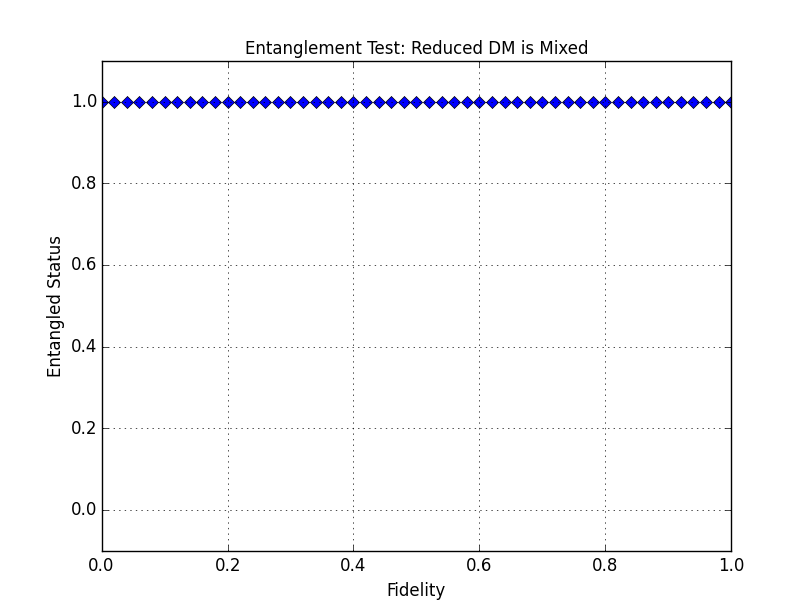
\includegraphics[scale=0.62]{figures/wernerstates-reducedmixed.png}
    \caption{Applying the entanglement test of mixedness of reduced density matrix to all possible Werner states.\newline \texttt{1 = True = Entangled,    0 = False = Separable}}
    \label{fig: Werner States: Mixedness of Reduced DM}
  \end{center}
\end{figure}

We can see that this test is failing to differentiate between separable and entangled states, showing all Werner states as entangled. This is in contrast to the time evolution example where we were dealing with a pure state. Hence we can conclude that this entanglement test is only good for pure states.

\subsubsection{Entropy of Entanglement}

\begin{figure}[H]
  \begin{center}
    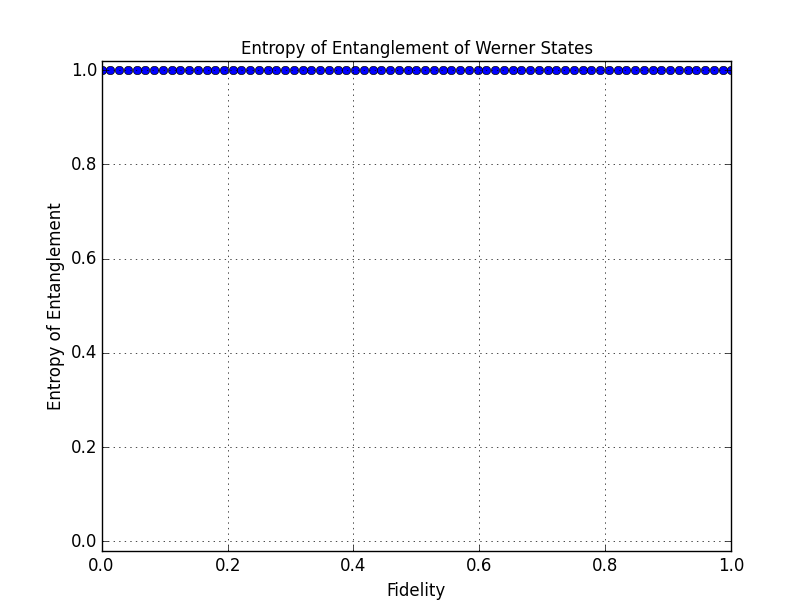
\includegraphics[scale=0.62]{figures/wernerstates-entropyentg.png}
    \caption{Entropy of Entanglement for all possible Werner states.}
    \label{fig: Werner States: Entropy of Entanglement}
  \end{center}
\end{figure}
We can see that this measure is failing to differentiate between separable and entangled states, showing maximal entanglement for all Werner states. This is due to the dependence of this measure on mixedness of the reduced density matrix, which makes it unable to identify states that are already mixed. Entropy of entanglement is good only as a measure of entanglement for pure states.
\newline
\par However, there are still a number of entanglement tests and measures that work with pure states as well as mixed states. The following are some of those tests and measures.


\subsubsection{The Peres-Horodecki Criterion}

\begin{figure}[H]
  \begin{center}
    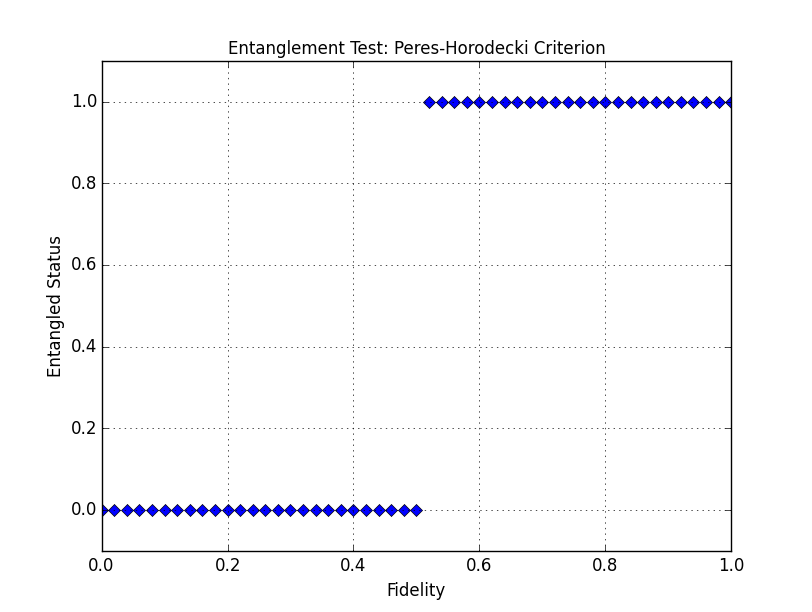
\includegraphics[scale=0.62]{figures/wernerstates-phcriterion.png}
    \caption{Applying the Peres-Horodecki criterion to all possible Werner states.\newline \texttt{1 = True = Entangled,    0 = False = Separable}}
    \label{fig: Werner States: Peres-Horodecki Criterion}
  \end{center}
\end{figure}

\par We can see that the Peres-Horodecki criterion is working as a reliable entanglement witness and showing Werner states with $F>1/2$ as entangled. It worked well for pure states in the Hamiltonian evolution case and it is also working for mixed states in the case of Werner states. This shows that the Peres-Horodecki criterion is a general entanglement witness which works well for pure as well as mixed states.


\subsubsection{Negativity and Logarithmic Negativity}

\begin{figure}[H]
  \begin{center}
    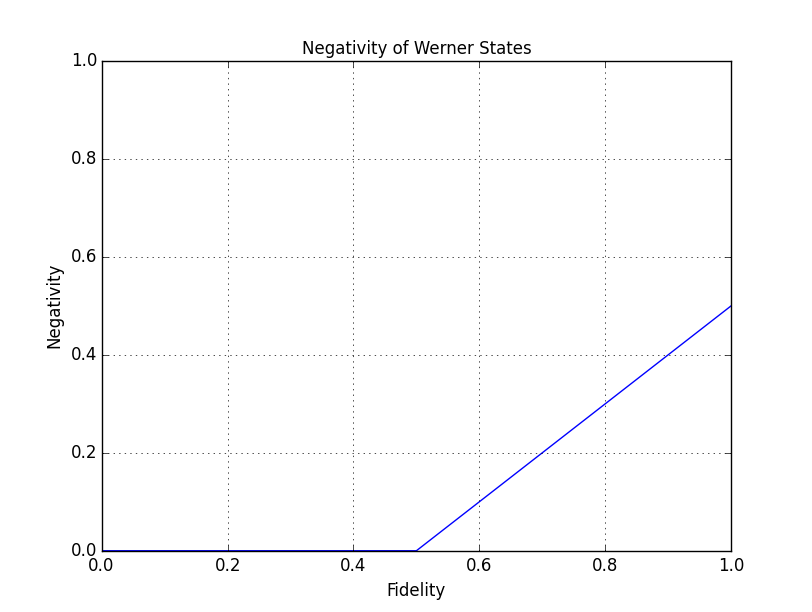
\includegraphics[scale=0.62]{figures/wernerstates-negativity.png}
    \caption{Negativity of Werner states for all possible values of singlet fidelity.}
    \label{fig: Werner States: Negativity}
  \end{center}
\end{figure}

We see that negativity starts increasing after $F=1/2$ and goes to the maximum value of 0.5 showing the state for $F=1$ as maximally entangled. This shows that negativity is a reliable measure of entanglement for both pure and mixed states.

\begin{figure}[H]
  \begin{center}
    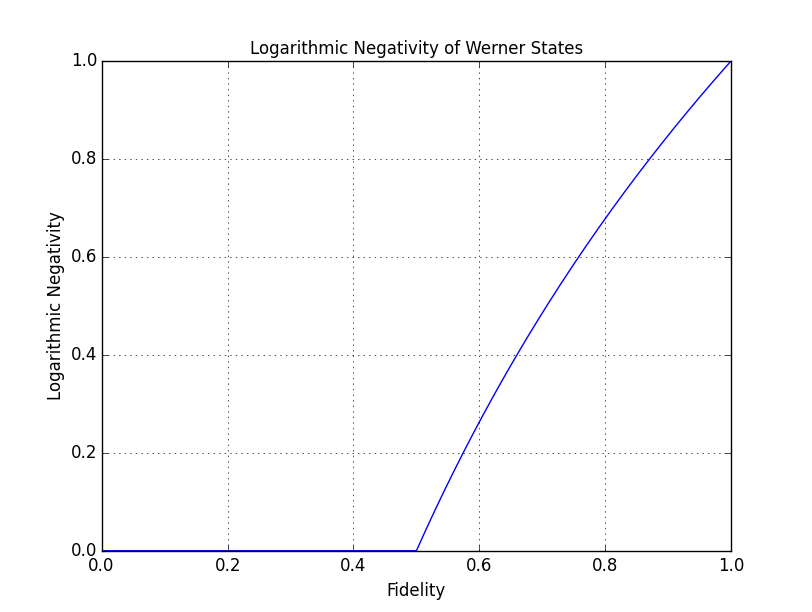
\includegraphics[scale=0.62]{figures/wernerstates-logneg.png}
    \caption{Logarithmic Negativity of Werner states for all possible values of singlet fidelity.}
    \label{fig: Werner States: Logarithmic Negativity}
  \end{center}
\end{figure}

As with negativity, logarithmic negativity also starts increasing after $F=1/2$ and reaches its maximum value for $F=1$. This shows that logarithmic negativity is also a good measure of entanglement for both pure and mixed states.


\subsubsection{Concurrence}

\begin{figure}[H]
  \begin{center}
    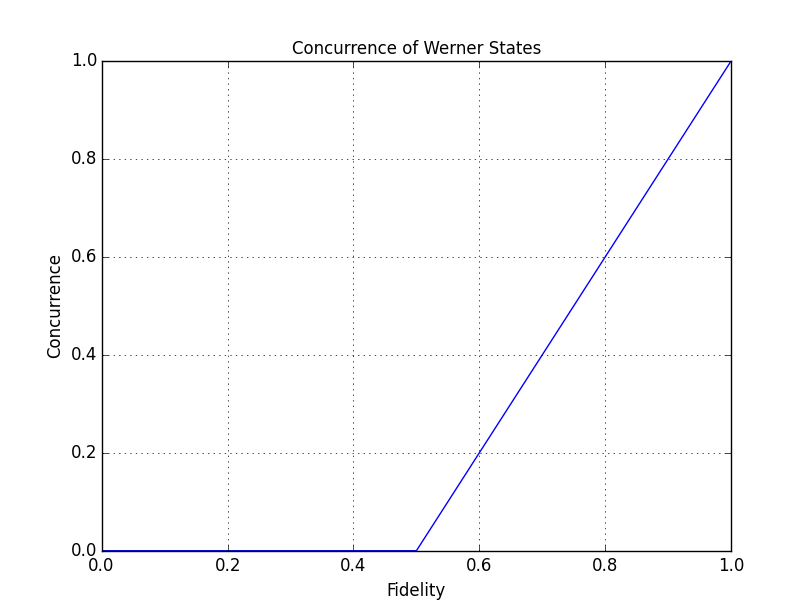
\includegraphics[scale=0.62]{figures/wernerstates-concurrence.png}
    \caption{Concurrence of Werner states for all possible values of singlet fidelity. The states start getting entangled after singlet fidelity exceeds $1/2$ and reach maximum entanglement for fidelity $F=1$.}
    \label{fig: Werner States: Concurrence}
  \end{center}
\end{figure}
We see that concurrence stays 0 for $F \leq 1/2$ when the states are disentangled. It starts increasing after $F$ exceeds $1/2$ and reaches its maximum value 1 for the maximally entangled state at $F=1$. This indicates that concurrence works for mixed states too and is a reliable measure of entanglement for both pure and mixed states.


\section{A Note About Optimizations}
QuTiP has a number of tricks available to make the functions much faster than our current implementation. However, since this project deals with the initial phase of implementing QI functions, we have not dwelled on the problem of speed optimizations. Rather we have focused primarily on implementing as many QI functions as possible. Later works on the subject can add the goal of making them faster.

